\chapter{Soluzione proposta}
In questo capitolo viene presentata la soluzione proposta per la rilevazione di disservizi nella connettivit\`a di reti locali.
Si analizza brevemente l'architettura del software sviluppato per poi fornirne una descrizione dettagliata della sua implementazione e del software utilizzato nello sviluppo.

\section{Architettura}
L'architettura della soluzione proposta \'e principalmente suddivisa in due parti come mostrato in figura \ref{fig:solproposta}: %FIGURA
\begin{itemize}

\item ArpScanner, una libreria che implementa un'operazione di ARP \cite{rfc826} scan, utilizzata per fornire una metrica del round-trip time (RTT) ed associare ad indirizzi IPv4 nella rete locale i rispettivi indirizzi MAC.
Bench\`e l'utilizzo di questa libreria sia facoltativo, nei capitoli successivi si mostrer\`a come i risultati ottenuti dall'operazione di ARP scan migliorino l'accuratezza della ricostruzione della topologia Wi-Fi.
\item WiFi-Topology, una libreria che, dopo aver catturato pacchetti di traffico di rete ed ottenuto i risultati dell' ARP scan, analizza i frame ricevuti e li utilizza per ricostruire una topologia della rete Wi-Fi fornendo valori di bont\`a del segnale.
Questa libreria \'e in grado di ricostruire topologie di reti sia in modalit\`a di cattura attiva o da file di cattura.
\end{itemize}

Le operazioni di cattura di pacchetti in entrambe le librerie sviluppate sono effettuate utilizzando l'API Pcap \cite{pcap}.
In particolare, nella libreria di ARP scanning vengono catturati frame di tipo Ethernet II mentre nella libreria per la ricostruzione della topologia di una rete i frame catturati sono di tipo 802.11.

\begin{figure}[!htb]
	\centering
	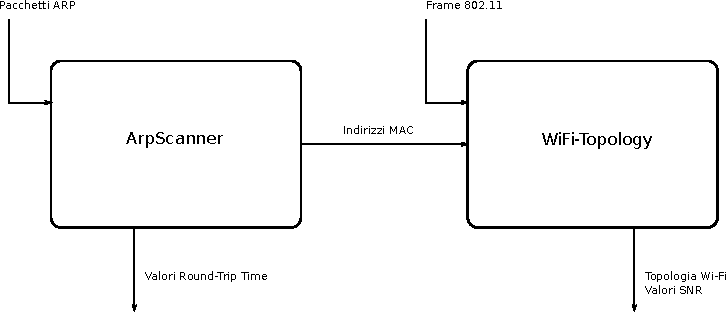
\includegraphics{images/drawingarchitettura.pdf}%img4.pdf}
	\caption{Architettura soluzione proposta}
	\label{fig:solproposta}
\end{figure}


Si discutono ora le strutture logiche delle due librerie sviluppate.

La libreria di ARP scan viene implementata utilizzando due librerie ausiliarie per le operazioni di invio e cattura pacchetti: dnet e libpcap.
La prima viene utilizzata per inviare i pacchetti ARP nel range di IP della sottorete mentre la seconda per raccogliere le risposte da eventuali dispositivi connessi alla rete.
Questo tipo di implementazione prevede quindi che il dispositivo sia connesso alla rete che si vuole monitorare e costituisce la parte di monitoraggio attivo della soluzione proposta.
%I risultati ottenuti da queste operazioni, oltre a fornire misure utili al monitoraggio della rete, vengono poi utilizzati per .

\begin{figure}[!htb]
	\centering
	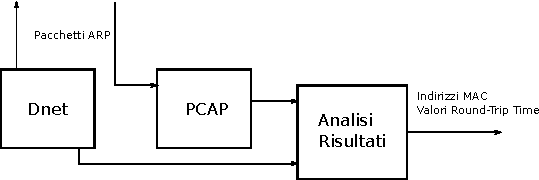
\includegraphics{images/drawingarpscanner.pdf}%img4.pdf}
	\caption{Struttura logica ArpScanner}
	\label{fig:ArpScanner}
\end{figure}


La libreria per la ricostruzione Wi-Fi, al contrario, effettua monitoraggio delle reti in modo passivo.
Non viene quindi inviato alcun tipo di pacchetto e le uniche azioni compiute sono quelle di cattura dei frame e la successiva analisi del traffico.
I risultati ottenuti dall'ARP scan possono essere utilizzati in quest'ultima operazione per aumentare l'accuratezza dei risultati forniti nella ricostruzione della topologia Wi-Fi.

\begin{figure}[!htb]
	\centering
	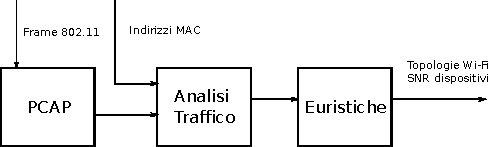
\includegraphics{images/drawingwifitopology.pdf}%img4.pdf}
	\caption{Struttura logica WiFi-Topology}
	\label{fig:WiFi-Topology}
\end{figure}


Poich\`e si vuole implementare questo tipo di soluzione su dispositivi con risorse di calcolo e memoria limitate si \'e prestata particolare attenzione al tipo di strutture utilizzate ed operazioni effettuate dalle librerie sviluppate.
In aggiunta, la soluzione proposta vuole limitare l'impatto prestazionale a cui viene sottoposta la rete durante le operazioni di monitoraggio.

Essendo la libreria ArpScanner l'unica ad implementare un tipo di monitoraggio attivo, l'unica operazione che pu\`o avere un impatto sulle prestazioni di rete \'e quella di invio dei pacchetti ARP.
Questa libreria non present\`a per\`o particolari richieste di calcolo o memoria dato il numero generalmente ristretto di dispositivi appartenenti ad una rete domestica ed ai pochi dati associati ad essi mediante l'operazione di arp scanning.

Al contrario, la libreria WiFi-Topology non ha alcun impatto sulle prestazioni della rete in esame poich\`e il tipo di monitoraggio effettuato \'e puramente passivo.
Il grande numero di pacchetti che viene catturato ed il numero di device presenti nelle vicinanze rendono questo tipo di analisi pi\`u dispendiosa dal punto di vista della memoria utilizzata.

\newpage
%Perche'


\section{Implementazione}
Si presentano brevemente, prima dei dettagli implementativi della libreria per la ricostruzione topologica della rete, il funzionamento della libreria utilizzata per la cattura dei pacchetti Pcap e quella implementata per effettuare ARP scanning.

Le librerie sono state sviluppate utilizzando il linguaggio di programmazione C++, un linguaggio nato come miglioramento del C, che permette l'uso del paradigma ad oggetti ed il controllo dell'utente della gestione della memoria.
Queste due caratteristiche hanno permesso di utilizzare puntatori per l'analisi dei frame catturati tramite la libreria libpcap e, allo stesso tempo, incapsulare i risultati dell'analisi in appropriati oggetti.

Inoltre, l'utilizzo del linguaggio C++ permette l'uso senza wrapper della libreria di cattura pacchetti libpcap, poich\`e questa \'e scritta in C.


 %questo ha permesso di combinare l'uso di costrutti ad alto livello come gli oggetti e l'accesso ai frame catturati tramite puntatori.

\subsection{Pcap}

Sviluppata da Tcpdump, libpcap  \'e una libreria scritta in linguaggio C che permette la cattura ed il filtraggio di pacchetti di rete.
La scelta di questa libreria si \'e basata su tre principali aspetti:
\begin{itemize}
	\item Facilit\`a d'uso: libpcap offre astrazioni ad alto livello per la cattura ed il filtraggio di pacchetti di rete.
	\item Filtraggio dei pacchetti: mediante la compilazione di un filter, \'e possibile catturare solo i pacchetti di rete di interesse per l'applicazione.  
	\item Compatibilit\`a: la libreria, oltre ad essere disponibile per la maggior parte dei sistemi operativi moderni, presenta numerosi wrapper per essere integrata in linguaggi di programmazione diversi dal C.
\end{itemize}
Di seguito si descrivono i passi necessari ad effettuare una cattura utilizzando libpcap:
\begin{enumerate}
	\item Scelta dell'interfaccia da utilizzare per la cattura.
	\item Inizializzazione dell'interfaccia e dei parametri della sessione.
	\item Creazione e compilazione del filtro da utilizzare per catturare i pacchetti desiderati. 
	\item Ciclo di ascolto in cui vengono analizzati, uno ad uno, i pacchetti catturati.
	\item Chiusura della sessione di cattura.
\end{enumerate}

%\newpage

\subsection{ARP Scan}

La libreria di ARP scan sviluppata permette la scoperta di tutti i dispositivi all'interno della rete locale.
Questa operazione viene effettuata inviando un numero di pacchetti ARP ad ogni possibile indirizzo IPv4 presente nella sottorete per poi, utilizzando libpcap, riceverne eventuali riscontri.

Il risultato ottenuto \'e un'associazione tra indirizzo IP ed indirizzo media access control (MAC), un indirizzo fisico univoco assegnato ad ogni scheda di rete dal proprio produttore.
L'indirizzo MAC cos\`i ottenuto verr\`a poi utilizzato per fornire una maggiore accuratezza nella ricostruzione della topologia Wi-Fi della rete locale in esame.

Sebbene questo sia il motivo principale di implementazione della libreria, \'e inoltre possibile ricavare una misura del round-trip time verso ogni dispositivo connesso alla rete, in modo analogo al ping attraverso richieste ICMP.
A differenza di quest'ultimo che pu\`o essere ignorato da alcuni tipi di dispositivi, utilizzando l'ARP ping con un numero di pacchetti appropriato \'e possibile ricevere riscontro da tutti i dispositivi attualmente connessi alla rete locale.
In particolare, i dispositivi che tendono ad ignorare questo tipo di richieste sono quelli di tipo mobile come smartphone e tablet nei momenti di non utilizzo da parte dell'utente.

Bench\`e ci siano gi\`a diverse implementazioni funzionanti per i sistemi operativi pi\`u utilizzati, si \'e deciso di sviluppare una libreria basilare che svolga solo le operazioni necessarie per la ricostruzione topologica della rete.
Si \'e cercato  in questo modo di limitare l'utilizzo di risorse e fornire una soluzione la cui implementazione \'e indipendente dal sistema operativo e basata solamente sull'uso di libpcap.

\newpage

%La libreria \'e stata scritta utilizzando il linguaggio di programmazione C++  

%ARP
%Pcap
%monitor mode, svantaggi
%Tipi di messaggi che filtriamo
%MAC header
%Tipi op e tipi header
%Euristica

%ascolto Attivo / ascolto passivo
\subsection{WiFi-Topology}
Dopo aver introdotto nelle sezioni precedenti una vista dell'architettura, purch\`e basilare, e le librerie fondamentali per il funzionamento della soluzione proposta si discute ora l'implementazione della principale libreria sviluppata durante il tirocinio.

La ricostruzione della topologia Wi-Fi delle reti viene effettuata attraverso l'analisi del traffico originato dalle stazioni presenti nelle vicinanze del dispositivo su cui il software \'e in esecuzione.

Questo tipo di cattura, come descritto precedemente, \'e effettuata utilizzando la libreria libpcap che permette di utilizzare un'interfaccia di tipo Wi-Fi in una particolare modalit\`a, chiamata monitor mode, di cui si espone di seguito il funzionamento.

\subsubsection{Monitor mode}
La cattura in monitor mode, o RFMON (Radio Frequency MONitor), permette ad una interfaccia di rete wireless di catturare tutto il traffico passante per un canale Wi-Fi.

In questa modalit\`a una scheda di rete non \'e associata ad alcun access point o rete ad-hoc e si pone in uno stato di ascolto in maniera completamente trasparente ad altri dispositivi wireless presenti nelle vicinanze.
Per effettuare ci\`o non vengono rispettati i normali comportamenti di una stazione operante con il protocollo 802.11, come ad esempio l'invio di ACK descritto nel secondo capitolo.
Di conseguenza, in questa modalit\`a, il dispositivo perde la possibilit\`a di trasmettere dati ed il suo utilizzo \'e ristretto ad un singolo canale wireless.
Un'altra limitazione in questo tipo di cattura riguarda il mancato controllo di errori nei pacchetti catturati, effettuato normalmente con un controllo di ridondanza ciclico (CRC).

Nonostante gli svantaggi elencati, questo tipo di modalit\`a trova molto utilizzo nella progrettazione di reti wireless, ad esempio per la scelta di un canale poco utilizzato al fine di diminuire interferenze tra stazioni, o nel cracking di reti protette con WEP .

Nello sviluppo della libreria questa modalit\`a \'e stata utilizzata per catturare diversi tipi di frame 802.11 trasmessi dai dispositivi nelle vicinanze.
Analizzando questo tipo di dati ed i valori di potenze di segnale forniti dal radiotap header \'e stato poi sviluppato un algoritmo per la ricostruzione della topologia delle reti Wi-Fi.
Per fornire una corretta analisi il controllo di ridondanza ciclico per i frame ricevuti  \'e stato integrato nella libreria sviluppata, in modo da poter evitare eventuali incoerenze tra la topologia ricostruita e quella effettiva.
In aggiunta, poich\`e la modalit\`a monitor dissocia la scheda di rete da un access point e cattura tutto il traffico passante per un canale, la libreria sviluppata non si limita a ricostruire una particolare rete di cui si \'e interessati ma fornisce una visione di tutte quelle nelle vicinanze.
Per sopperire all'impossibilit\`a di ascoltare su pi\`u di un canale si \'e fatto uso di uno script per effettuare channel hopping, in modo da poter catturare traffico per qualche secondo su ciascun canale.

Il compromesso principale dell'uso della monitor mode resta quello di dover dedicare completamente un'interfaccia Wi-Fi alla cattura dei frame dissociandola dalla rete locale che si vuole monitorare.
Per questo motivo, su dispositivi dotati di una sola scheda di rete, non \'e possibile mantenere costantemente attiva la cattura perdendo quindi la possibilit\`a di assistere a cambi nella topologia di rete in tempo reale. 
Un recente studio \cite{zanetti2010non} ha evidenziato come sia possibile virtualizzare, senza perdita di prestazioni, interfacce per la cattura di traffico in modalit\`a promiscua o, come in questo caso, in monitor mode.

Nella prossime sezioni vengono introdotti in dettaglio i frame catturati in questa modalit\`a e come essi sono utilizzati per la ricostruzione della topologia della rete.

\subsubsection{MAC Frame}

Prima di mostrare come avviene l'analisi del traffico si introduce la struttura generale dei frame catturati tramite monitor mode ed i tipi rilevanti al funzionamento della libreria.
Nei protocolli di rete wireless 802.11 un MAC frame, rappresentato in figura \ref{fig:macframe}, \'e composto da campi comuni a tutti i tipi di frame e da campi specifici ad alcuni di essi.

\begin{figure}[!htb]
	\centering
	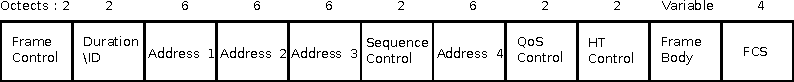
\includegraphics{images/img5.pdf}
	\caption{MAC frame}
	\label{fig:macframe}
\end{figure}

Un frame 802.11 contiene quindi un MAC header di lunghezza pari a 34 byte, un body di lunghezza variabile in base al tipo di frame catturato ed infine un campo di 4 byte per il controllo degli errori.

Di seguito si fornisce una breve descrizione di tutti i campi presenti nel MAC header, in particolare di quelli utilizzati durante l'implementazione della libreria:

\newpage

\begin{itemize}
	\item Frame Control: 2 byte che forniscono informazioni sul tipo del frame.
	\item Duration/ID: 2 byte che indicano alle stazioni la durata della trasmessione e viene usato per inizializzare il valore del NAV introdotto nel secondo capitolo.
	\item Address 1-2-3-4: 6 ottetti che identificano unicamente un dispositivo tramite   indirizzo MAC.
	\item Sequence Control: diviso in due campi di 12 e 4 bit che indicano, rispettivamente, il numero di sequenza ed il numero del frammento del pacchetto.
	\item QoS Control: 2 byte che identificano i parametri QoS in un frame di dati.
	\item HT Control: 2 byte aggiunti dallo standard 802.11n.
	\item Frame Body: campo di lunghezza e tipo variabile, payload del frame.
	\item FCS: 4 byte di frame check sequence, un codice di rilevazione di errore.
\end{itemize}

I campi interessanti per la ricostruzione della topologia di una rete includono il frame control, gli indirizzi MAC, il body del frame ed il FCS.
In particolare, nella figura \ref{fig:framecontrolfields}, possiamo osservare come il frame control sia suddiviso in 11 sottocampi.

\begin{figure}[!htb]
	\centering
	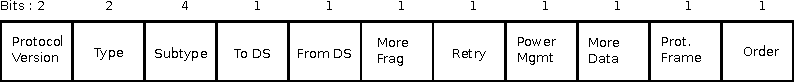
\includegraphics{images/img6.pdf}
	\caption{Frame Control Fields}
	\label{fig:framecontrolfields}
\end{figure}

Il primo campo, protocol version, indica la versione del protocollo 802.11 in uso dal frame ed \'e sempre pari a 0 poich\`e attualmente esiste una sola versione di questo protocollo.

Il secondo e terzo campo del frame control indicano invece il tipo e sottotipo del frame ricevuto.Questo tipo di informazione \'e fondamentale per una corretta analisi poich\`e a diversi tipi e sottotipi di frame corrispondono diversi campi nel frame body.

Data la lunghezza pari a 2 bit, un frame nello standard 802.11 pu\`o essere suddiviso in quattro categorie di tipo diverse, che a loro volta possono contenere sedici sottocategorie codificate con 4 bit:
\begin{itemize}
	\item 00- Management Frame: forniscono informazioni sullo stato della rete e sono utilizzati per la connessione e disconnessione di dispositivi.
	\item 01- Control Frame: assistono la trasmissione di data frame e per amministrare l'accesso al mezzo al mezzo trasmissivo.
	\item 10- Data Frame: contengono dati di protocolli di livello superiore all'interno del loro body.
	\item 11- Reserved: tipo di frame riservato e non utilizzato nello standard 802.11.
\end{itemize}

L'utilizzo e il tipo di analisi effettuata su questi tipi di frame ed i loro sottotipi verr\`a introdotto in apposite sezioni.

I successivi due campi del frame control, To DS e From DS, sono di particolare importanza per lo studio effettuato sulla ricostruzione della topologia di rete.
Questi due bit possono essere utilizzati per determinare quando un frame \'e immesso nel mezzo trasmissivo wireless e quando, invece, ne esce.

Di seguito si evidenziano i possibili valori di verit\`a dei due campi:

\begin{itemize}
	\item To DS=0, From DS=0 : il frame non deve lasciare il mezzo trasmissivo, valore generalmente associato a tipi di frame come: management e control.
	\item To DS=0, From DS=1 : il frame proviene da un access point e sta entrando nel mezzo trasmissivo wireless.
	\item To DS=1, From DS=0 : il frame proviene da un client e sta uscendo dal mezzo trasmissivo wireless.
	\item To DS=1, From DS=1 : il frame \'e destinato ad un'altra rete wireless.
\end{itemize}

Accoppiando questo tipo di analisi del mezzo trasmissivo con i valori di segnale ottenuti tramite Radiotap \'e possibile rilevare anche eventuali dispositivi connessi ad un access point via cavo, purch\`e il traffico analizzato contenga un cambio di mezzo trasmissivo.

Un esempio, che sar\`a discusso anche nel prossimo capitolo, potrebbe essere quello di un router collegato via cavo ad un access point ed un numero di dispositivi connessi in Wi-Fi a quest'ultimo.

\newpage

\subsubsection{MAC Address}

Un MAC address \'e un identificatore unico associato ad un'interfaccia di rete dal proprio costruttore e viene utilizzato nel protocollo 802.11 per l'instradamento dei frame.
L'indirizzo \'e formato da una struttura di 48 bit divisa in 6 ottetti, come mostrato in figura \ref{fig:macaddress}.
%Guidelines for Use of Extended Unique Identifier (EUI), Organizationally Unique Identifier (OUI), and Company ID
Per mantenere l'unicit\`a tutte le schede di rete prodotte \'e stato introdotto uno standard, chiamato EUI-48 e gestito dalla IEEE, che divide l'indirizzo MAC in due parti:
\begin{itemize}
	\item Organisationally Unique Identifier (OUI): identifica unicamente un produttore di schede di rete ed \'e assegnato dalla IEEE.
	\item Network Interface Controller (NIC): identifica unicamente una determinata scheda di rete e viene assegnata dal prodottore.
\end{itemize}

\begin{figure}[!htb]
	\centering
	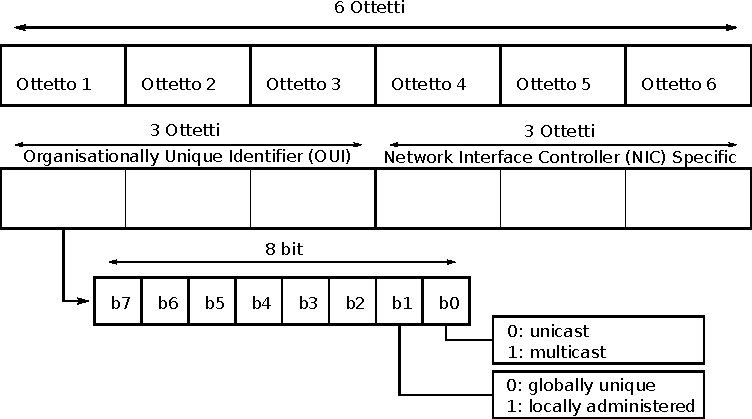
\includegraphics{images/img7.pdf}
	\caption{Mac Address}
	\label{fig:macaddress}
\end{figure}

In aggiunta, un indirizzo MAC pu\`o essere universalmente (UAA) o localmente (LAA) assegnato.
Questa diversificazione viene effettuata attraverso il valore del secondo bit meno signficativo del primo ottetto.
Per quanto riguarda gli indirizzi UAA, questo bit viene posto a 0 ed il valore del primo ottetto \'e pari a quello del OUI.
Al contrario, un valore del bit pari ad 1 identifica un indirizzo LAA che viene generalmente assegnato da eventuali amministratori di rete.

La differenziazione del tipo di trasmissione in unicast e multicast avviene in maniera simile, in questo caso l'identificazione avviene mediante il bit meno significativo del primo ottetto.

Un valore pari a 0 equivale ad una trasmissione unicast mentre un valore pari ad 1 una trasmissione di tipo multicast.
Infine, l'indirizzo di broadcast \'e ottenuto ponendo un valore pari ad 1 ad ogni bit dell'indirizzo MAC.

Come visto precedentemente, un MAC header \'e costituito da quattro indirizzi MAC il cui valore e significato varia in base al tipo di frame ed ai valori To DS e From DS.
Gli indirizzi possono essere dei seguenti tipi:
\begin{itemize}
	\item Receiver Address (RA): indirizzo della stazione che riceve il frame.
	\item Transmitter Address (TA): indirizzo della stazione che trasmette il frame.
	\item Basic Service Set Identifier (BSSID): indirizzo dell'access point della rete.
	\item Destination Address (DA): indirizzo di destinazione finale del frame.
	\item Source Address (SA): indirizzo sorgente del frame.
\end{itemize}

Nella figura \ref{table:addressvalue} si mostrano le varie combinazioni che gli indirizzi MAC possono rappresentare in base ai valori presenti nel frame control.

\begin{table}[h]
\centering
\begin{tabular}{| l | l | l | l | l | l |}
	\hline 
	To DS  & From DS & Address 1 & Address 2 & Address 3 & Address 4\\ \hline
	 0 & 0 & RA=DA & TA=SA & BSSID & N/A \\ \hline
     0 & 1 & RA=DA & TA=BSSID & SA & N/A\\ \hline
	 1 & 0 & RA=BSSID & TA=SA & DA & N/A\\ \hline
	 1 & 1 & RA & TA & DA & SA\\ \hline
\end{tabular}
%\end{flushright}
\centering
\caption{Tabella uso indirizzi MAC }
\label{table:addressvalue}
\end{table}

%Aggiungere ref
%Accennare qui indirizzo locale repeater?

\newpage

\subsubsection{Management Frame}

I frame di tipo management vengono utilizzati dalle stazioni e dall'access point per regolare l'accesso e disconnessione alla rete WLAN.
Questo tipo di frame permette, durante la parte di analisi del traffico, di identificare gli access point  attivi ed eventuali dispositivi che stiano cercando di accedervi.
%Bench\`e i sottotipi definiti per questo tipo di frame siano 16 si elencano, in tabella \ref{table:managementframes}, solo quelli effettivamente utilizzati dalla libreria per la costruzione topologica della rete.

%\begin{table}[h]
\begin{wraptable}{r}{8cm}
\centering
\begin{tabular}{| l | l |}
	\hline
	Subtype  & Descrizione \\ \hline
	%0000 & Association Request \\ \hline
	0001	 & Association Response 	\\ \hline
  %  0010	 & Reassociation Request \\ \hline
	%0011	 & Reassociation Response \\ \hline
	0100	 & Probe Request \\ \hline
	%0101	 & Probe Response \\ \hline
%	0110	& Timing Advertisement \\ \hline
	%0111	& Reserved \\ \hline
	1000 &	Beacon \\ \hline
	%1001	& ATIM \\ \hline
	1010	& Disassociation \\ \hline
	%1011	& Authentication \\ \hline
	1100	& Deauthentication \\ \hline
	%1101	& Action \\ \hline
	%1110	& Action No Ack (NACK) \\ \hline
	%1111	& Reserved \\ \hline 
\end{tabular}
%\end{flushright}
\centering
\caption{Sottotipi Mgmt Frame}
\label{table:managementframes}
%\end{table}
\end{wraptable}

Bench\`e i sottotipi definiti per questo tipo di frame siano 16 si elencano, in tabella \ref{table:managementframes}, solo quelli effettivamente utilizzati dalla libreria per la costruzione topologica della rete.

Il sottotipo di frame pi\`u interessante per questa operazione \'e quello di Beacon, che viene utilizzato dagli access point per annunciare la presenza di una rete WLAN alle stazioni vicine.

Nel frame body sono presenti 5 campi obbligatori:

\begin{itemize}
	\item Timestamp: 8 byte che indicano il tempo di attivit\`a dell'access point.
	\item Beacon Interval: 2 byte che indicano la frequenza di invio di un beacon frame.
	\item Capability Information: 2 byte utilizzati per specificare 
	funzionalit\`a aggiuntive dell'access point.
	\item	SSID: lunghezza variabile, identifica il nome logico di una rete WLAN.
	\item Supported Rates: specifica la velocit\`a in Mbps che la stazione offre.
\end{itemize}

La libreria utilizza il Beacon frame per determinare se il MAC address del mittente sia  un access point che avr\`a, eventualmente, una serie di dispositivi a lui connesso.
In aggiunta, analizzando il radiotap header di un Beacon frame \'e possibile fornire un quadro completo sui dettagli della rete che viene annunciata, in particolare: canale in uso, potenza del segnale.

Come intuibile dalla descrizione, i frame di Association Response, Disassociation e Deauthentication indicano connessioni e disconnessioni di dispositivi alla rete wireless.
In particolare i tipi di frame riguardanti le disconnessioni sono fondamentali per evitare di fornire una topologia della rete in cui vengano identificati come collegati dispositivi che non sono pi\`u appartenenti alla rete.
Nonostante la loro importanza, la frequenza con cui questi frame vengono analizzati dipende fortemente dal tipo di monitoraggio che si effettua: costante o ad istanti di tempo.

A differenza dei frame precedenti il Probe Request viene inviato da un dispositivo che si pone in cerca di reti WLAN a cui accedere e  la sua analisi avviene solo per misurare parametri di bont\`a del segnale poich\`e il dispositivo non \'e connesso a nessuna rete.

\subsubsection{Control Frame}

I frame di tipo control assistono l'invio di frame management e data, amministrando l'accesso al mezzo trasmissivo wireless.

Come evidente dalla tabella \ref{table:controlframes} i principali frame che vengono analizzati corrispondono a quelli introdotti nella presentazione di DCF nel secondo capitolo.
\begin{table}[h]
%\begin{wraptable}{r}{8cm}
\centering
\begin{tabular}{| l | l |}
	\hline
	Subtype  & Descrizione \\ \hline
	1001	 & Block Ack 	\\ \hline
	1011	 & RTS \\ \hline
	1100 &	CTS \\ \hline
	1101	& ACK \\ \hline
\end{tabular}
%\end{flushright}
\centering
\caption{Sottotipi Control Frame}
\label{table:controlframes}
%\end{table}
%\end{wraptable}
\end{table}

In questo tipo di frame, come specificato da DCF, non \'e presente un frame body.
Per questo motivo l'analisi dei control frame da parte della libreria \'e in grado di fornire solamente una relazione di connessione tra due indirizzi MAC e quindi due dispositivi.

\subsubsection{Data Frame}

I Data frame vengono utilizzati nel protocollo 802.11 per la trasmissione di dati provenienti da livelli superiori.

\begin{wraptable}{r}{8cm}
\centering
\begin{tabular}{| l | l |}
	\hline
	Subtype  & Descrizione \\ \hline
	0000	 & Null No Data 	\\ \hline
	0100	 & Data \\ \hline
	1000 &	QoS Data \\ \hline
	1100	& QoS Null No Data \\ \hline
\end{tabular}
%\end{flushright}
\centering
\caption{Sottotipi Data Frame}
\label{table:dataframes}
%\end{table}
\end{wraptable}

In tabella \ref{table:dataframes} si evidenziano i sottotipi di questo frame che vengono analizzati per la ricostruzione della topologia della rete WLAN.

La cattura e l'analisi di questi tipi di frame permette l'identificazione dei dispositivi su cui la trasmissione wireless termina o inizia.

Sfruttando questa informazione \'e quindi possibile identificare per ogni stazione che trasmette un frame il dispositivo a cui esso \'e collegato.

Come verr\`a esposto nella sezione successiva questo procedimento \'e fondamentale per la corretta rappresentazione della topologia di rete e permette di identificare il percorso dei frame inviati da un dispositivo anche in presenza di ripetitori Wi-Fi.

\subsubsection{Analisi ed euristica}

Il funzionamento della libreria pu\`o essere diviso in tre principali fasi delle quali si  spiega, nel dettaglio, il funzionamento:

\begin{enumerate}
	\item Cattura ed analisi dei frame 802.11.
	\item Ispezione degli indirizzi MAC dei dispositivi presenti e di eventuali access point. 
	\item Topologia risultante.
\end{enumerate}

La cattura dei frame 802.11, come precedentemente introdotto, viene effettuata mediante la libreria libpcap ed impostando la scheda di rete Wi-Fi in modalit\`a monitor.
Durante questa procedura, per ogni frame ricevuto dalla scheda di rete, vengono analizzati il radiotap header ed il MAC header.
In particolare, utilizzando il radiotap header, vengono estratte informazioni riguardanti la potenza del segnale della stazione che trasmette il frame ed il canale utilizzato per l'invio.

L'analisi del MAC header \'e cruciale per fornire una corretta ricostruzione della topologia di rete e comprende diversi controlli di correttezza.
In primis viene effettuato un controllo sul FCS per poter scartare tutti i frame corrotti che vengono catturati.
Se il pacchetto ricevuto \'e esente da errori, vengono successivamente analizzati gli indirizzi MAC in base al tipo e sottotipo di frame ricevuto.
In questo controllo vengono scartati tutti pacchetti di tipo data e control i cui indirizzi destinatari sono di tipo broadcast, poich\`e questi tipi di frame non forniscono informazioni su alcun dispositivo connesso.

Soddisfatti questi requisiti gli indirizzi MAC presenti nel frame vengono considerati dispositivi Wi-Fi di interesse e memorizzati per poi poter esser nuovamente ispezionati al termine del procedimento di cattura.

Nel caso in cui il dispositivo analizzato abbia trasmesso almeno un frame di tipo beacon, questo viene considerato come un access point.
\newpage
Per ogni dispositivo, in questo stadio dell'esecuzione, sono quindi noti i seguenti valori:
\begin{itemize}
	\item Canale, potenza e rumore dell'antenna.
	\item Indirizzo MAC.
	\item Lista di indirizzi MAC con cui il dispositivo interagisce.
	\item Nome della rete annunciata (se AP).
\end{itemize}

La fase successiva necessaria per la ricostruzione della topologia di rete consiste nell'associare eventuali indirizzi MAC virtuali e multicast ai rispettivi indirizzi globalmente assegnati.
Questo procedimento \'e necessario per evitare di includere nella topologia Wi-Fi indirizzi MAC che, in realt\`a, non appartengono a nessun dispositivo.
Non \'e affatto raro, infatti, l'utilizzo di indirizzi virtuali da parte di repeater ed access point per la trasmissione in rete o l'uso di multicast da parte di router per l'invio di frame a singoli dispositivi.
Il risultato ottenuto \'e un diretto collegamento tra un indirizzo virtuale al suo indirizzo globalmente assegnato, sia esso ottenuto mediante una precedente ARP scan o dalla cattura di frame 802.11.

Il passo successivo effettuato dalla libreria \'e quello di applicare un'euristica in grado di determinare se un dispositivo di rete abbia pi\`u di una antenna Wi-Fi ed in che modo queste vengano utilizzate.
Gli attuali access point presenti in commercio aderiscono allo standard 802.11AC e sono quindi provvisti di una moltitudine di antenne wireless.
Dopo lo studio di numerosi dispositivi di questo tipo si \'e formulata un'euristica coerente con i comportamenti osservati, basata sulla divisione dell'indirizzo MAC in due sezioni:la prima comprendente i primi cinque ottetti e la seconda il restante ottetto.
Infatti, gli indirizzi MAC delle varie antenne presenti in questo tipo di dispositivi sembrano essere sempre maggiori in valore rispetto all'indirizzo fornito dal produttore.
Considerando quindi tutti gli indirizzi MAC ottenuti dalla cattura di frame ed, eventualmente, anche dall'ARP scan si seleziona quello che presenta un valore minore nell'ultimo ottetto come l'indirizzo effettivo del dispositivo.

L'euristica presentata, in aggiunta a quella implementata per assegnare un indirizzo MAC globale ad uno localmente assegnato, risolve inoltre un altro problema emerso durante lo sviluppo della libreria riguardante l'utilizzo di indirizzi MAC da parte di repeater Wi-Fi.
Durante lo studio approntato sono stati infatti individuati due metodi di funzionamento dei repeater, anche in dispositivi la cui unica differenza risiedeva nel firmware installato.

Uno dei metodi in cui i repeater trattano il traffico \'e quello intuitivo in cui i frame inviati e ricevuti dai dispositivi associati vengono trasmessi in modo trasparente dal repeater stesso.
In questo caso l'indirizzo MAC del repeater viene incluso nel frame 802.11 come TA.

Il secondo metodo osservato consiste nell'uso da parte del repeater di diversi indirizzi MAC per ogni dispositivo ad esso connesso.
In particolare il MAC risultante \'e cos\`i definito: i primi tre ottetti corrispondono al LAA del repeater mentre gli ultimi tre ottetti corrispondono al NIC del dispositivo a lui connesso.
%Immagine
La validazione di questi tipi di euristiche \'e rimandata al capitolo successivo.

L'ultimo passo effettuato dalla libreria \'e quello di creare due strutture facili da interpretare che rappresentino la topologia di ogni rete Wi-Fi nelle vicinanze.

Una struttura contiene una lista di tutte le reti wireless, in particolare:

\begin{itemize}
	\item Indirizzo MAC dell'access point, canale della rete Wi-Fi, potenza segnale e rumore.
	\item Lista di indirizzi MAC dei dispositivi connessi alla rete, indicando se questi siano connessi direttamente all'access point o meno.
\end{itemize}

La seconda struttura contiene invece una lista di indirizzi tutti i dispositivi attivi nelle vicinanze ed un indirizzo a cui essi sono collegati, sia esso un access point o repeater, ed i valori di potenza segnale e rumore.

